
\subsection{Mappa}
Per la mappa è stato utilizzato \gmaps{} e l'implementazione è contenuta nel fragment \texttt{WaveHeatMapFragment}.

\subsubsection{Generazione cella}
Una cella della mappa rappresenta la misurazione di un'area quadrata\footnote{Esclusa la zona equatoriale, le celle appariranno rettangolari} e la dimensione di quest'ultima scala automaticamente in base al livello dello zoom.

Una cella è descritta dalle coordinate del vertice superiore sinistro (nord-ovest) e a partire da questa vengono calcolate le coordinate degli altri convertendo la dimensione della cella (in metri) in un offset da applicare a latitudine e longitudine.
Per questioni estetiche, gli offset sono approssimati in modo tale che tutte le righe siano allineate verticalmente (\cref{fig:tile_offset}).
\begin{figure}[H]
    \centering
    \begin{minipage}[b]{0.45\textwidth}
      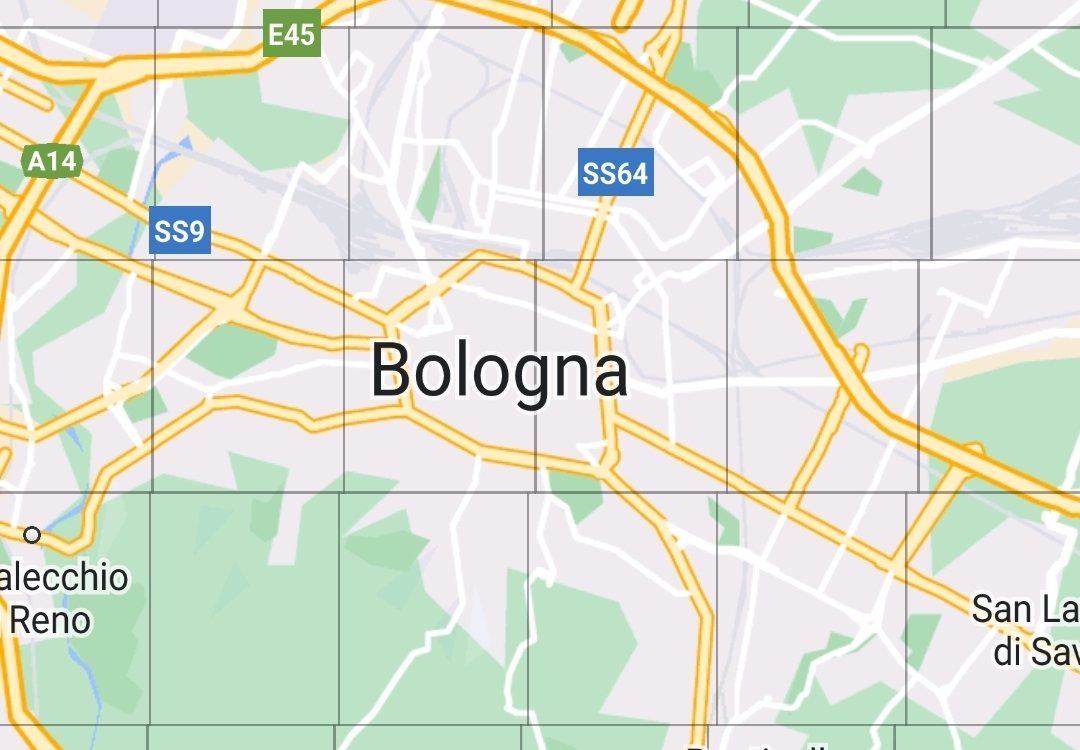
\includegraphics[width=\textwidth]{./img/tile_no_approx.jpg}
    \end{minipage}
    \hfill
    \begin{minipage}[b]{0.45\textwidth}
      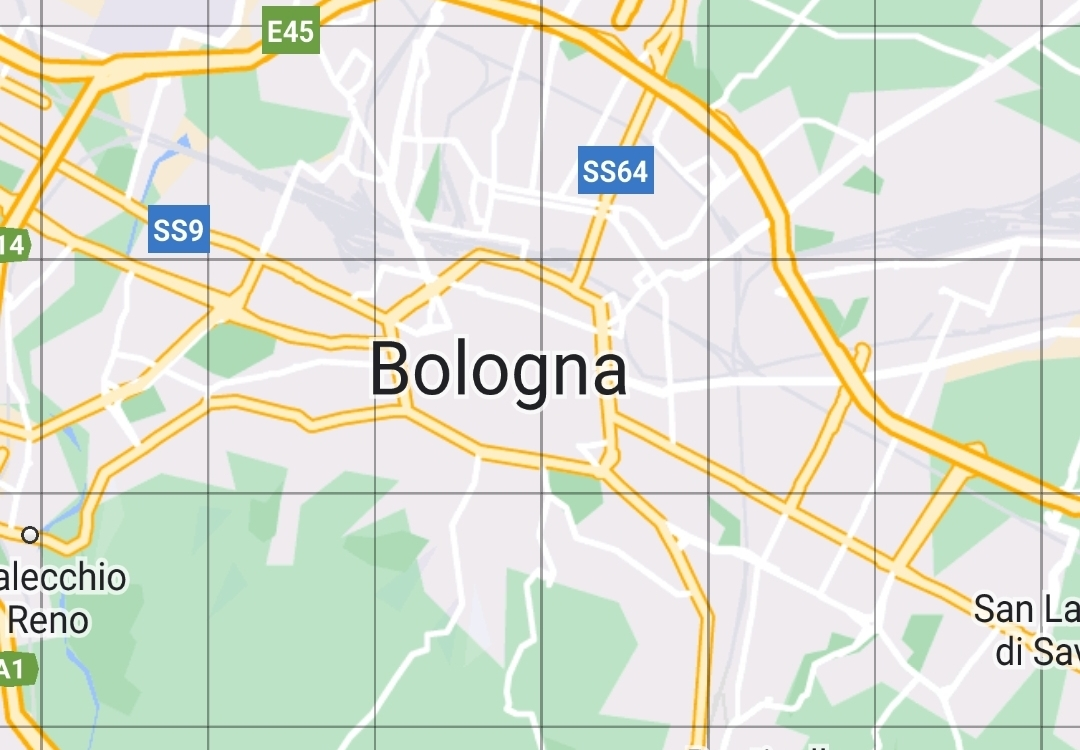
\includegraphics[width=\textwidth]{./img/tile_approx.jpg}
    \end{minipage}
    \caption{Offset calcolati in maniera precisa (sinistra) e approssimata (destra)} \label{fig:tile_offset}
\end{figure}

Il colore di una cella è determinato dal valore e dal tipo di misurazione, e viene impostato in formato HSV modificando il valore della tinta (hue).
Per ciascuna tipologia di misurazione sono specificati gli estremi del range di qualità e il numero di intervalli in cui suddividerlo.
La tinta è quindi determinata collocando il valore della misurazione in uno dei sotto-intervalli del range e selezionando come valore finale l'estremo inferiore (\cref{alg:hue}).

\begin{algorithm}[H]
  \caption{Tinta di una cella}\label{alg:hue}
  \SetAlgoLined
  \SetKwProg{Fn}{fun}{}{end}
  \Fn{\textup{\texttt{{getHue(measure, measure\_range=[$a$, $b$], hue\_range=[$0$, $150$], n\_ranges)}}}}{
    $\texttt{hue} \gets \text{\texttt{measure} scalata da \texttt{measure\_range} a \texttt{hue\_range}}$\\
    $\texttt{hue} \gets \text{\texttt{hue} discretizzata in \texttt{hue\_range} suddiviso in \texttt{n\_ranges} valori}$\\
    return \texttt{hue}
  }
\end{algorithm}

Infine, per ogni cella è presente un'etichetta contenente il valore della misurazione. Poiché \gmaps{} non permette di inserire esplicitamente del testo nella mappa, l'implementazione prevede di generare l'etichetta come un'immagine che viene poi impostata come icona di un marker. Inoltre, in caso di necessità, la dimensione del testo viene scalata per far in modo che rientri nei limiti della cella.


\subsubsection{Generazione griglia}
La griglia è composta da celle generate relativamente ad una posizione di riferimento. In particolare, in fase di inizializzazione viene designata come cella di riferimento quella che pone la posizione dell'utente al centro e in base a questa è possibile determinare la posizione di tutte le altre celle della mappa. 

Nello specifico, date delle coordinate $(\texttt{pos}_{\texttt{lat}}, \texttt{pos}_{\texttt{lon}})$, per determinare la cella che la contiene si calcola il numero di celle da saltare rispetto a quella di riferimento: 
\begin{equation*}
    \texttt{to\_skip\_tiles}_\texttt{lat} =
        \lceil \frac{\texttt{pos}_{\texttt{lat}} - \texttt{center\_top\_left}_{\texttt{lat}}}{\texttt{latitudeOffset(tile\_length\_meters)}} \rceil
\end{equation*}
\begin{equation*}
    \texttt{to\_skip\_tiles}_\texttt{lon} =
        \lfloor \frac{\texttt{pos}_{\texttt{lon}} - \texttt{center\_top\_left}_{\texttt{lon}}}{\texttt{longitudeOffset(tile\_length\_meters)}} \rfloor
\end{equation*}
Le coordinate del vertice superiore sinistro della cella che contiene $(\texttt{pos}_{\texttt{lat}}, \texttt{pos}_{\texttt{lon}})$ sono quindi:
\begin{equation*}
    \texttt{tile}_\texttt{lat} = \texttt{center\_top\_left}_{\texttt{lat}} + (\texttt{to\_skip\_tiles}_\texttt{lat} \cdot \texttt{latitudeOffset(tile\_length\_meters)})
\end{equation*}
\begin{equation*}
    \texttt{tile}_\texttt{lon} = \texttt{center\_top\_left}_{\texttt{lon}} + (\texttt{to\_skip\_tiles}_\texttt{lon} \cdot \texttt{longitudeOffset(tile\_length\_meters)})
\end{equation*}

Con questo approccio, ogni volta che viene spostata la visuale della mappa, la griglia viene generata iterando a partire dalle coordinate dell'angolo nord-ovest visibile dello schermo, fino a raggiungere l'angolo sud-est. 

In aggiunta, per maggiore efficienza, si tiene traccia delle celle generate in modo da evitare di dover ridisegnare l'intera area visibile ad ogni movimento della mappa. Questo meccanismo viene resettato quando viene cambiato il livello di zoom, in quanto tutte le celle già presenti diventano obsolete e vengono necessariamente cancellate.